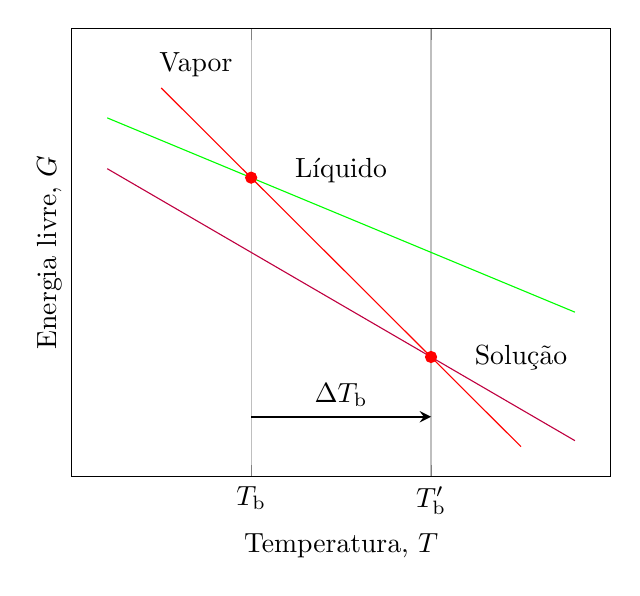
\begin{tikzpicture}
\begin{axis}
    [
        grid = major,
        ylabel = {Energia livre, $G$},
        xlabel = {Temperatura, $T$},
        domain = 0.2:2.8,
        xmin = 0, xmax = 3,
        ymin = -20, ymax = 10,
        xtick= {1, 2}, 
        xticklabels={$T_\mathrm{b}$, $T_\mathrm{b}^\prime$},
        ytick=\empty,
    ]
    \addplot [ purple ]
        { 2-7*x };
    \node [anchor = south] at (axis cs:2.5, -13.5) 
        { Solução };

    \addplot [ green ]
        { 5-5*x };
    \node [anchor = south] at (axis cs:1.5, -1) 
        { Líquido };

    \addplot [ red, domain=0.5:2.5 ]
        { 12-12*x };
    \node [anchor = north east] at (axis cs:0.95, 9) 
        { Vapor };

    \addplot [ mark=*, color=red, only marks ] coordinates
        { (1, 0) (2, -12) };

    \draw [ draw=black, thick, -stealth ]
        (axis cs: 1, -16) -- node [above] {$\Delta T_\mathrm{b}$}
        (axis cs: 2, -16);
\end{axis}
\end{tikzpicture}
